%!TEX root = ../documentation.tex
\chapter{Training}
\label{ch:training}

Nach der Auswahl der Modelle kann der Trainingsprozess beginnen. Dazu betrachten wir zunächst die generelle Methodik, welche wir angewendet haben.
Ziel war es ein möglichst gutes Modell mit einer hohen Genauigkeit zu erhalten.

\section{Methodik}

\subsection{Early Stopping}

Mithilfe von Early Stopping regularisieren wir das Training. Damit soll Overfitting vermieden und somit eine hohe Generelisierungsfähigkeit sichergestellt werden.\\
Dies geschieht indem das Training beendet wird sobald eine konvergierte Genauigkeit festgestellt wird.

\subsection{Hyperparameter Tuning}

Durch schrittweises Anpassen der Parameter wird auf eine bessere Leistung des Modells hingearbeitet. Diesen Prozess bezeichnet man als Hyperparameter Tuning.\\
Angepasst haben wir neben der Lernrate und dem Zerfall dieser auch die Batch-Größe.

\subsection{Transfer Learning}

Als Transfer Learning wird die Übertragung von bereits gelernten Gewichten bezeichnet. Durch diese Methode kann ein Netzwerk mit einem großen Datensatz trainiert werden und anschließend können die gelernten Features auf ähnliche Problemstellungen angewandt werden.

\section{ResNet152 Modell}

Wir wenden bei diesem Modell das beschriebene Transfer Learning an. Die vortrainierten Gewichte stammen aus dem Training mit dem ImageNet Datensatz.\\
Für das ResNet Modell haben wir als Verlustfunktion die kategorische Kreuzentropie gewählt. Zusammen mit dem Adam Optimizer (Lernrate 0.01, Zerfall 1e-5) erhalten wir die folgenden Ergebnisse.

\begin{figure}[H]
    \centering
    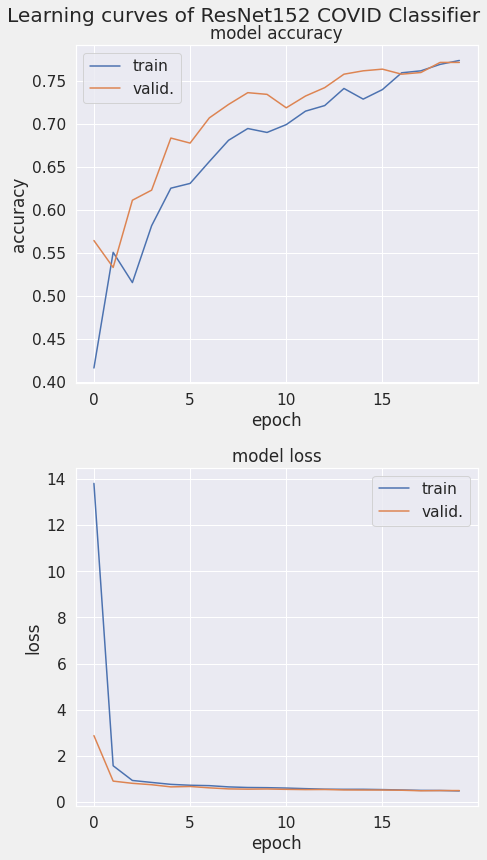
\includegraphics[width=0.5\textwidth]{../results/ResNet152_curves.png}
    \caption{}
\end{figure}

\pagebreak

\section{SqueezeNet}

Bei dem SqueezeNet Modell kommt ebenfalls kategorische Kreuzentropie und der Adam Optimizer zum Einsatz. Allerdings nutzen wir hier eine geringere Lernrate von 0.00001 bei gleichbleibendem Zerfall von 1e-5.

\subsection{Drei Klassen}

Durch ein Training auf Basis von drei Klassen erhalten wir die folgenden Ergebnisse.

\begin{figure}[H]
    \centering
    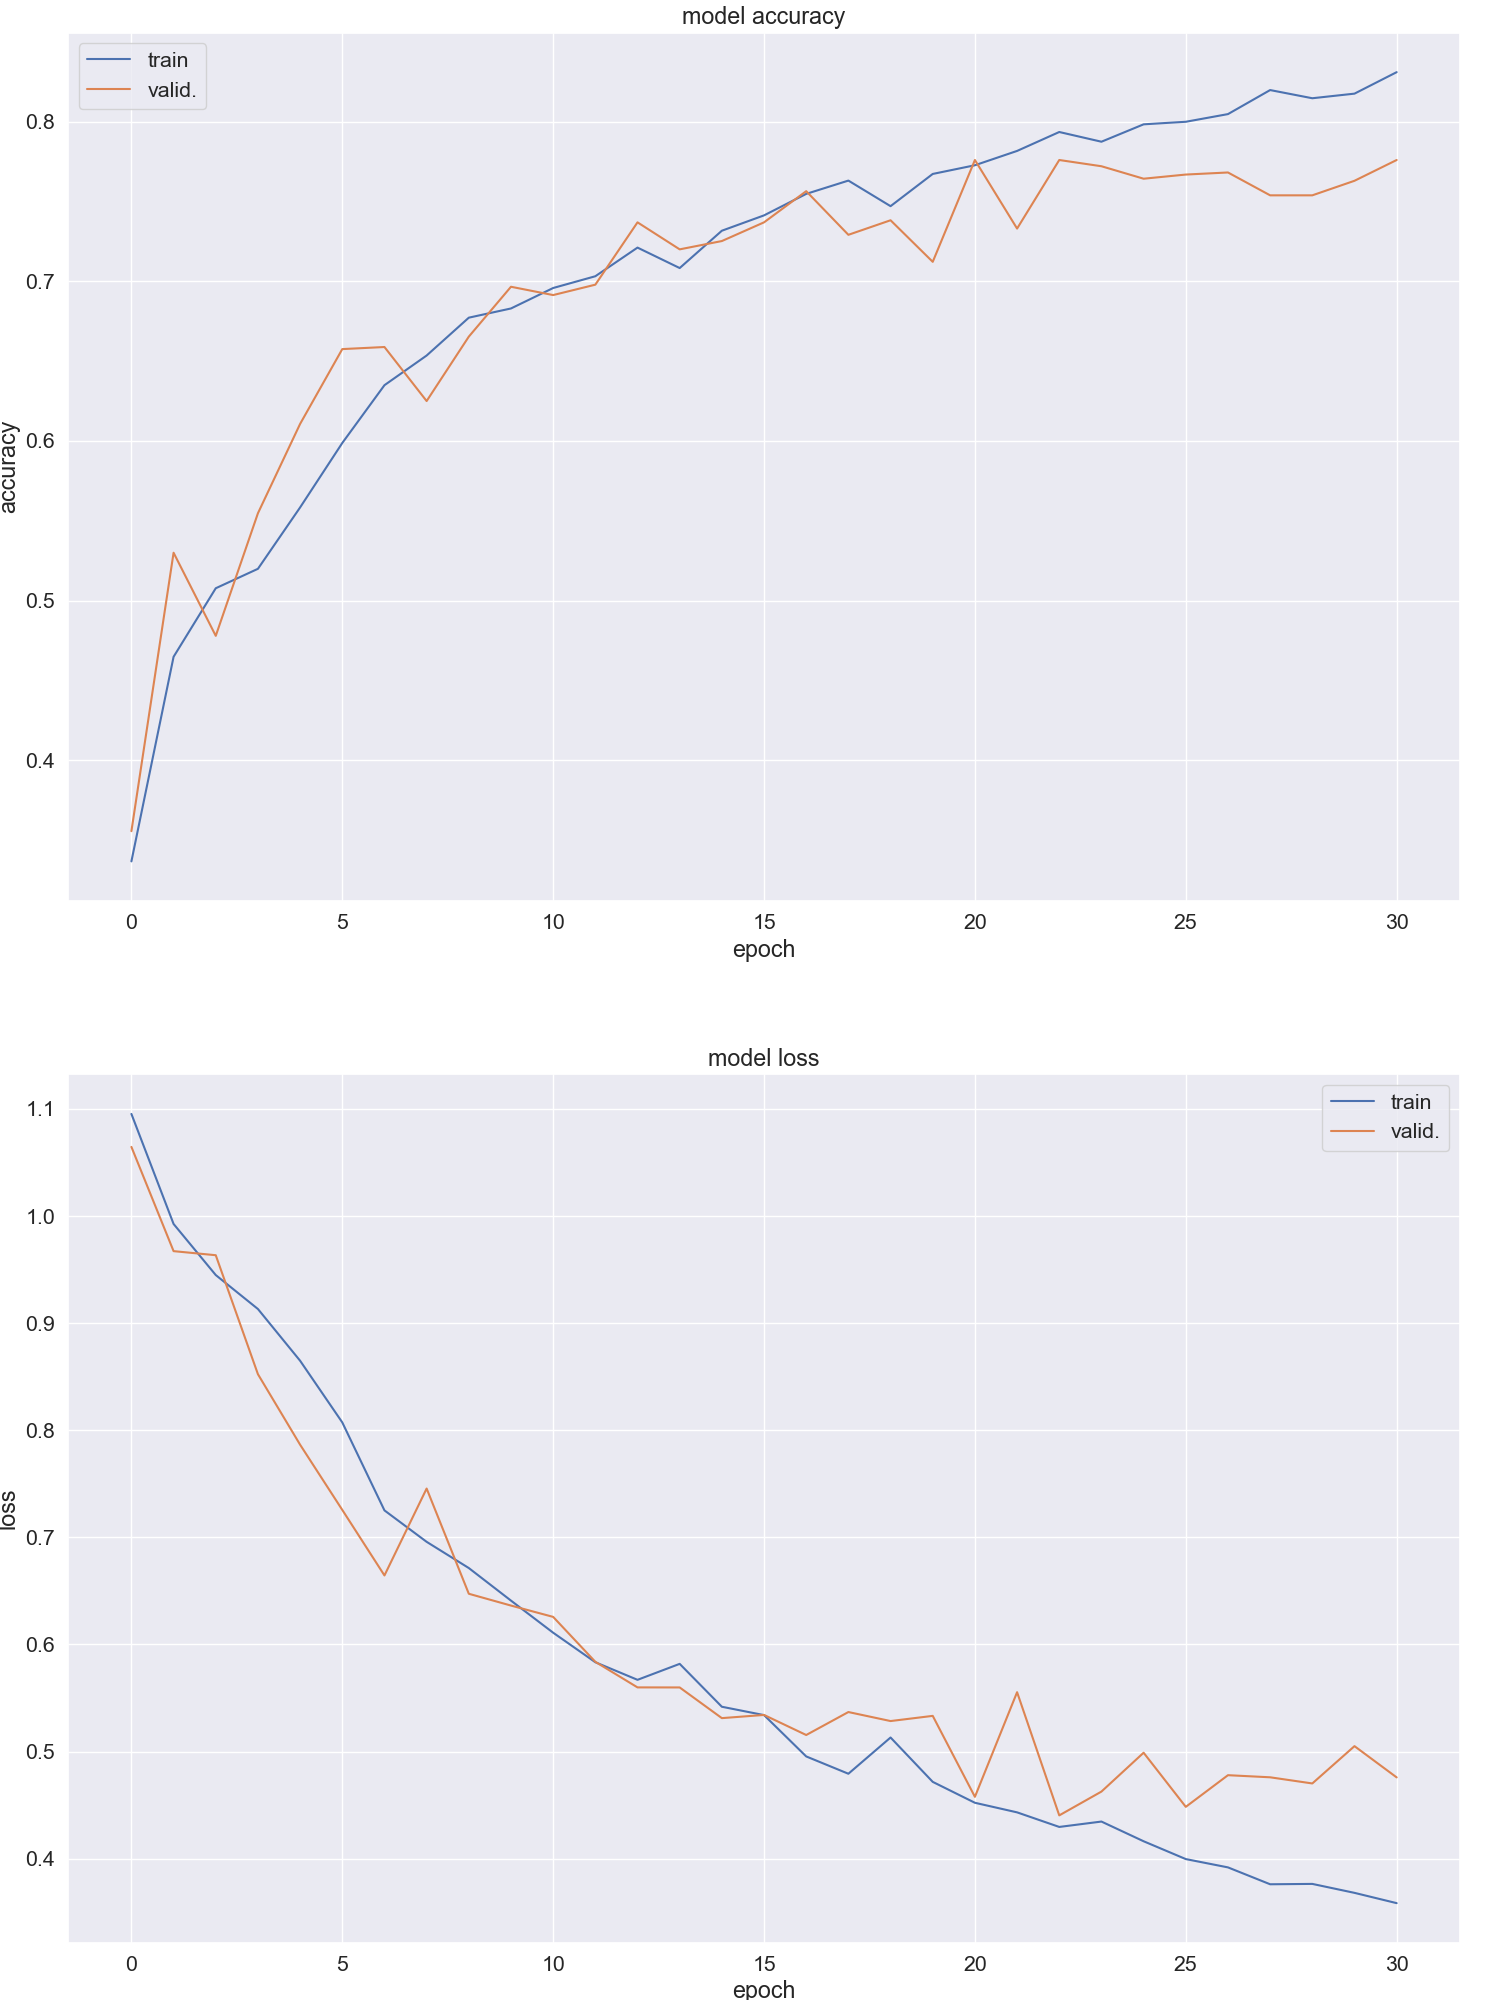
\includegraphics[width=0.75\textwidth]{../results/SqueezeNet_curves.png}
    \caption{}
\end{figure}

\subsection{Binäre Klassifizierung}

Wir haben zusätzlich eine Version des SqueezeNet Modells implementiert, welche eine binäre Klassifizierung vornimmt. Hier werden die Bilder in die Klassen "COVID-19" und "nicht COVID-19" unterteilt.

\begin{figure}[H]
    \centering
    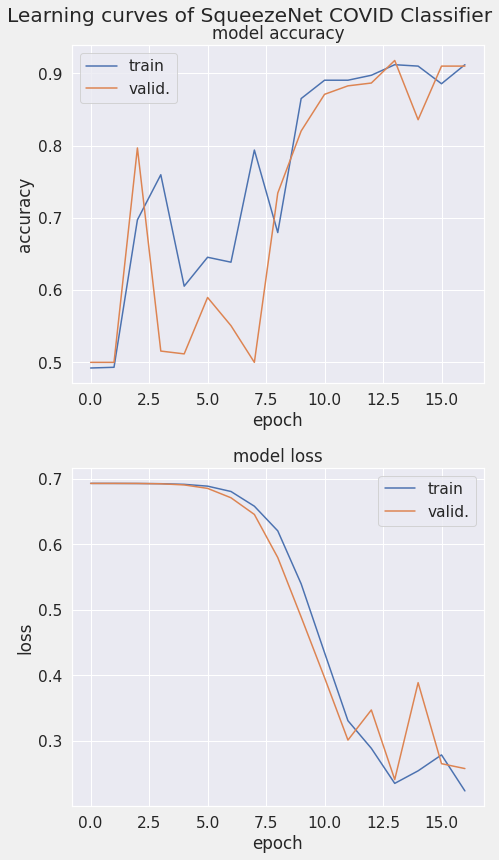
\includegraphics[width=0.5\textwidth]{../results/Binary_SqueezeNet_curves.png}
    \caption{}
\end{figure}